\documentclass[doctor]{snuece-bs}

\usepackage{biblatex}
\addbibresource{10-bibliography.tex}

\title[korean]{AmslerTouch: 노인황반변성 증상의 정량적 자가진단을 지원하는 암슬러 그리드 애플리케이션 설계}
\title[english]{AmslerTouch: Self-testing Amsler Grid Application for Supporting a Quantitative Report of Age-related Macular Degeneration Symptoms}


\author[korean]{신 동 훈}
\author[english]{DONGHOON SHIN}
\author[nospace]{신동훈}


\advisor{서 종 모}

\submissiondeadline{2021년 6월}
\examinationdate{2021년 8월}

\gradyear[english]{AUGUST 2022}
\gradyear[korean]{2022년 8월}


\begin{document}
\renewcommand{\baselinestretch}{1.5}

\selectfont

\begin{abstract}
	\par
	Age-related macular degeneration (AMD) is a progressive chronic disease that is led by damage in the macula. Due to its irreversible characteristics and disastrous effects on the patients, a precise diagnosis of the symptoms is extremely important. Yet, paper-based Amsler Grid, the most prevalent testing method, is highly limited in that it requires the indirect report of patients and quantitative reporting is difficult. To address this, I propose AmslerTouch, a touch-based Amsler-testing web app that supports patients to self-report AMD symptoms. Based on the reflection on the proposed system, I also discuss future enhancements.
	\vfill
	\begin{minipage}[t][20mm][b]{\textwidth}
		{\bfseries Keywords}: Age-related Macular Degeneration, Amsler Grid, Healthcare\\
		{\bfseries Student number}: 2016-16578\\
	\end{minipage}
	
\end{abstract}

\changepage{5mm}{}{}{}{}{}{}{}{-5mm}

\makelists

\chapter{INTRODUCTION}

Age-related macular degeneration (AMD) is a progressive chronic disease that is led by the damage in the macula~\cite{lim2012age}. According to Jeon et al., AMD is a highly prevalent disease in the society, where 6.62\% of South Korean population are suffering from the symptoms of AMD~\cite{park2014age}. It is widely known that the symptom often accompanies a disastrous symptoms, such as blurred vision or vision loss~\cite{lim2012age}. In addition to its detrimental effects on the vision itself, older adults with AMD are also prone to be affected psychologically, such as being depressed from the isolation from the society led by the symptom~\cite{rovner2007preventing}.

To date, however, little or no effective treatment for treating AMD exists~\cite{wong2011prevention}. Although some promising approaches such as stem cell implant have been proposed~\cite{carr2013development}, these methods are still yet to be widely applied. Thus, considering that it is almost impossible to revert once the degeneration is exacerbated, the most feasible and cost-effective management of AMD is to prevent further development of symptoms~\cite{al2017recent}, implying the necessity of the early detection and precise diagnosis of AMD.

As such, the importance of precise diagnosis has been highly emphasized so far. Yet, most of the diagnosis of AMD are limited in precisely reporting the region of issue. Specifically, patients and practitioners who conduct Amsler grid testing, the most prevalent AMD testing since 1940s, often suffer from the communicative issues, thus limiting the validity of the test~\cite{schuchard1993validity}. Heavily relying on the indirect, verbal report of patients, the regions of issue are often inexactly reported, making such symptoms difficult to be accurately managed.

In order to address such an issue, I propose a novel application of self-reporting symptoms of AMD with Amsler grid. Specifically, based on the literature review of AMD and the symptoms that are led by the disease, I developed AmslerTouch, a touch-based Amsler-testing web app that supports patients to self-report AMD symptoms. AmslerTouch supports users to precisely annotate regions of symptoms. As such, I aimed to faciliated decision making of practitioners with the quantitative report of AMD symptoms with a widely-available tablet device. Based on the reflection on AmslerTouch, I also discuss possible enhancements and future works.

\chapter{BODY}

\section{Method}
This study was built upon the previous works in the field of human-computer interaction (HCI) that dealt with diagnosing AMD symptoms with aids of computing systems. Based on these implications of these approaches and the understanding of frequent symptoms reported by ophthalmologists, I propose our touch-based interactive Amsler grid testing app.


\section{Literature Review}

\subsection{Diagnosis and Management of Symptoms with Aid of Computers}

With the advent and distribution of personal computing devices, previous studies have explored and proposed various computer-based techniques that supports diagnosis of various diseases and disorders. For example, Shin and his colleagues TalkingBoogie, a mobile app that supports ad hoc notes of communicative issues that children with non-verbal developmental disabilities show~\cite{shin2020talkingboogie}. Salai and Baillie developed a mobile application for recording overactive bladder symptoms~\cite{salai2019wee}.

\subsection{Age-related Macular Degeneration (AMD)}

\subsubsection{Distortion}

\begin{figure}[h!]
    \centering
    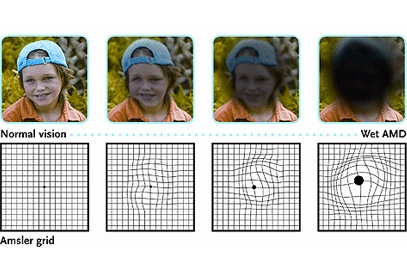
\includegraphics[width=0.6\linewidth]{figure/symptoms.jpg}
    \caption{Distortion}
    \label{fig:my_label}
\end{figure}

\subsection{Computer-based AMD Diagnosis}

Previous studies in the field of Human-computer interaction, bioengineering, and health informatics have explored several techniques that support medical practitioners and patients to diagnose symptoms of AMD in computers. Noting that paper-based AMD testing had been shown unsuccessful in terms of precise diagnosis~\cite{fine1986earliest, roy1985vision}, these studies emphasized the feasibility of computer-based approach for the precise and quantitative report of symptoms.

For example, Loewenstein et al. proposed MCPT, a system that supports patients to draw their region of symptoms on the computer~\cite{loewenstein2003replacing}. With basic input sources such as ordinary mouse and keyboard, these researchers sought to support a precise computer-based diagnosis. Mohaghegh and his colleagues developed a wearable system for diagnosing AMD symptoms~\cite{mohaghegh2016wearable}. They developed NGRID, a diagnosis system with a head-mounted device to support more precise diagnosis of AMD. In addition to such approaches, recent advent of 3D technologies made it possible to diagnose with 3D screen and glasses~\cite{kim2020novel}.

\begin{table}[htbp]
	\begin{center}
		\begin{tabular}{|c|c|} \hline
			Name & Description\\ \hline
			\hline {\sc MCPT~\cite{loewenstein2003replacing}} & Drawing on the computer with ordinary mouse and keyboard\\
			\hline {\sc NGRID~\cite{mohaghegh2016wearable}} & Head-mounted Amsler-grid app\\
			\hline {\sc 3D Test~\cite{kim2020novel}} & Implemented with 3D screen and polarized glasses\\
			\hline
		\end{tabular}
		\caption{Examples of AMD Diagnosis apps}
		\label{tab1}
	\end{center}
\end{table}

As such, previous researchers were successful in exploring design spaces of novel diagnosis systems and proposing them. Yet, these approaches are limited in its efficiency and generalizability, since (i) they only made use of simple input devices that might not be sufficient in terms of accuracy or (ii) the techniques required costly devices that are not easily available. With recent distribution of touch-based tablets, I found that these devices might give people a great opportunity to precisely note regions of symptom without purchasing any costly device. Thus, in this study, I propose an AMD diagnosis app that lets users easily utilize within their hand-held devices.

\section{Design of AmslerTouch}
In this section, I discuss my design decisions for the touch-based Amsler grid app. Speficil
\subsection{Implementation}

AmslerTouch is implemented as a web application, targeted to both touch interaction and mouse click. I developed the program using Svelte~\cite{svelte}, a Javascript framework for developing a web application. After being developed, the program was deployed on Google Firebase and the source code later became available at GitHub\footnote{https://github.com/donghoon-io/AmslerTouch}.

While developing AmslerTouch, I utilized the following third-party libraries to enhance the usability of the system. All of these libraries are properly used under the license of each library:

\begin{itemize}
    \item \textbf{Notus-svelte~\cite{notus-svelte}}: A theme for svelte web app. This library is used for designing an interface
    \item \textbf{React canvas draw~\cite{react-canvas-draw}}: A Javascript tool for drawing regions. I modified the library to draw a circle and fill the circle with Gaussian filter
\end{itemize}

\printbibliography

\begin{summary}
	\par
	
	노인 황반변성 (Age-related macular degeneration; AMD)은 황반 내 손상에 의해 야기되는 진행성 만성 질환이다. 치료가 어려운 해당 질병의 특성과 환자에 미치는 만성적인 영향 때문에 AMD는 증상에 대한 정확한 진단이 매우 중요하다. 하지만, 전세계적으로 AMD를 진단하기 위해 가장 널리 사용되는 테스트 방법 중 하나인 종이 기반 Amsler grid는 환자가 간접적으로 증상에 대해 말하는 방식으로 진행되고, 정량적 보고가 어렵다는 점에서 매우 제한적이다. 이를 해결하기 위해, 본 연구에서는 AmslerTouch를 제안한다. AmslerTouch 터치 기반의 Amsler grid 웹 앱으로, 환자가 AMD 증상을 자가 보고할 수 있도록 지원하는 프로그램이다. 제안된 시스템을 바탕으로, 향후 해당 시스템을 발전시킬 수 있는 방안 또한 제언한다.
	\vfill
	\begin{minipage}[t][20mm][b]{\textwidth}
		{\bfseries 주요어}: 노인 황반변성, 암슬러 그리드, 헬스케어\\
		{\bfseries 학번}: 2016-16578\\
	\end{minipage}
\end{summary}
\acknowledgement{
	\par
	I would like to thank all the people for supporting me throughout my undergraduate studies.
}
\end{document}
